\begin{figure}[H]
\centering
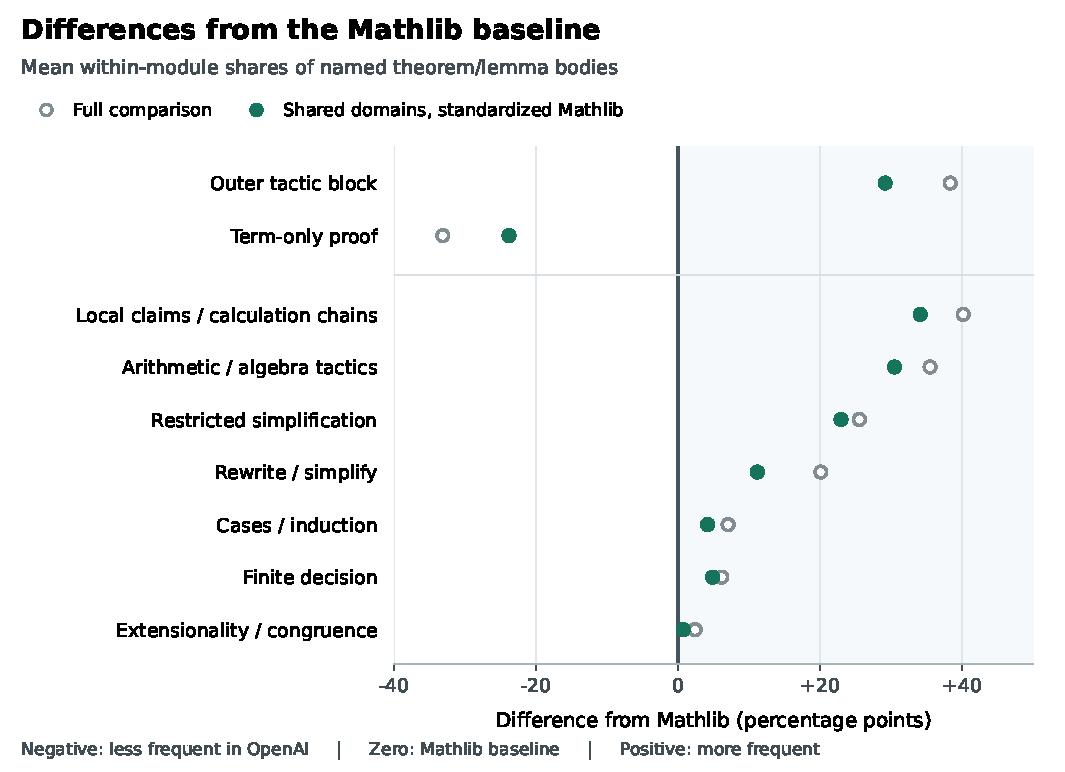
\includegraphics[width=\textwidth]{figures/method-shift.pdf}
\caption{OpenAI minus Mathlib differences in written proof-feature
prevalence, in percentage points. Zero denotes equal prevalence;
positive values indicate greater prevalence in the OpenAI sample.
Hollow markers compare all proof-bearing modules (784 OpenAI and
7,348 Mathlib). Green markers retain 735 OpenAI modules in 18 shared
domains and reweight Mathlib to the OpenAI domain shares. Both markers
lie at the same height for each feature and denote separate estimates
of the difference from Mathlib. Both comparisons average within-module
proof-body shares; features overlap except for the proof-mode
categories. The figure shows point estimates. Table~\ref{tab:profile}
reports absolute rates and 95\% OpenAI sampling intervals for selected
features in the full comparison. Table~\ref{tab:joint-profile} adds joint
subject and proof-length standardization.}
\label{fig:method-shift}
\end{figure}
